\chapter{Практическая часть}

Проанализировать работу приведенных программ и объяснить результат их работы.

\section{Задание \No{}1}
Реализовать загружаемый модуль ядра, который при загрузке записывает в системный журнал сообщение о запущенных процессах. Модуль должен собираться при помощи Make-файла.
Загружаемый модуль должен содержать:
\begin{itemize}
\item указание лицензии GPL;
\item указание автора.
\end{itemize}
Текст первой программы:

\lstset{language=c}
\begin{lstlisting}[caption=Текст программы первого задания]
#include <linux/module.h>
#include <linux/init.h>
#include <linux/kernel.h>
#include <linux/sched.h>
#include <linux/init_task.h>

MODULE_LICENSE("GPL");
MODULE_AUTHOR("Alexander Kupry");
MODULE_DESCRIPTION("lab_03_task_1");

static int __init my_module_init(void)
{
    printk(KERN_INFO "My module is loaded\n");

    struct task_struct *task = &init_task;

    do
    {
        printk(KERN_INFO "My module: process %s -- %d, parent: %s -- %d\n",
            task->comm, task->pid, task->parent->comm, task->parent->pid);
    }
    while ((task = next_task(task)) != &init_task);


    printk(KERN_INFO "My module: process current: %s -- %d, parent: %s -- %d\n",
        current->comm, current->pid, current->parent->comm, current->parent->pid);

    return 0;
}

static void __exit my_module_exit(void)
{
    printk(KERN_INFO "My module is unloaded\n");
}

module_init(my_module_init);
module_exit(my_module_exit);
\end{lstlisting}

Результат сборки загружаемого модуля ядра md1 при помощи утилиты make:

\begin{figure}[H]
    \centering
    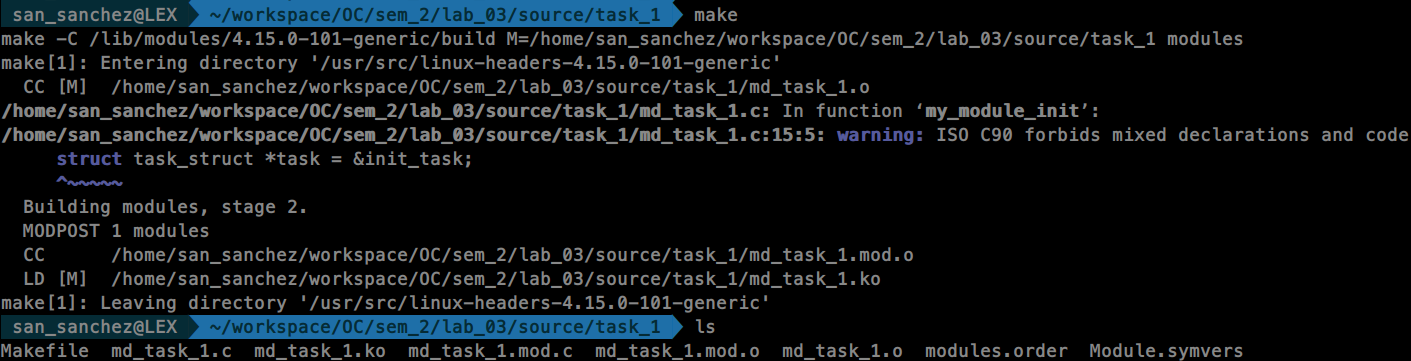
\includegraphics[scale=0.34]{data/image/task_1_new.png}
    \caption{Скришот результата работы make.}
\end{figure}

Загрузка модуля и демонстрация успешной загрузки:

\begin{figure}[H]
    \centering
    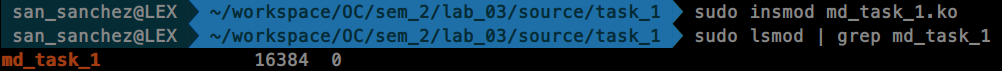
\includegraphics[scale=0.45]{data/image/task_1_2.png}
    \caption{Скришот результата работы lsmod.}
\end{figure}

Вывод dmesg:

\begin{figure}[H]
    \centering
    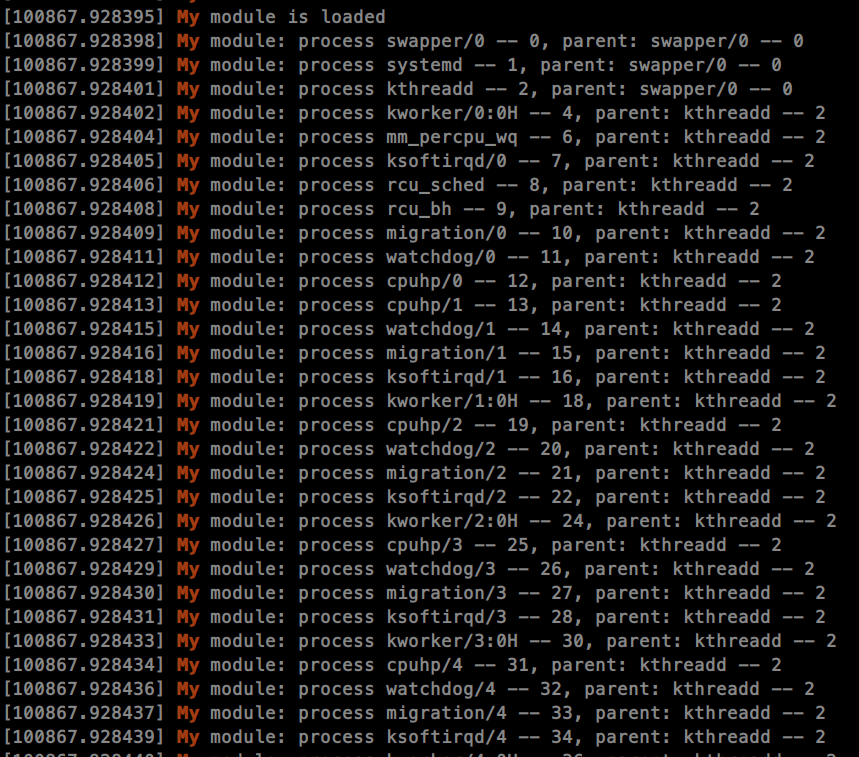
\includegraphics[scale=0.5]{data/image/task_1_3.png}
    \caption{Скришот результата работы dmesg.}
\end{figure}

Демонстрация успешной выгрузки модуля.

\begin{figure}[H]
    \centering
    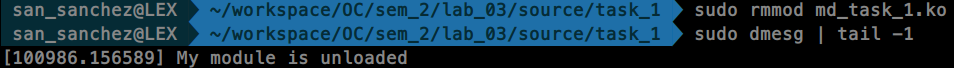
\includegraphics[scale=0.5]{data/image/task_1_4.png}
    \caption{Скришот результата работы rmmod.}
\end{figure}

\section{Задание \No{}2}

Реализовать три загружаемых модуля ядра:
\begin{itemize}
    \item Вызываемыи модуль md1;
    \item Вызывающии модуль md2;
    \item «Отладочныи» модуль md3.
\end{itemize}
Каждыи загружаемыи модуль должен содержать:
\begin{itemize}
    \item Указание лицензии GPL
    \item Указание автора
\end{itemize}
Загружаемые модули должны собираться при помощи Make-фаила (сборка командои make). Вызов каждои функции модуля должен сопровождаться записью в системныи журнал информации, какая функция какого модуля была вызвана.

\textbf{Модуль md1}

Модуль md1 демонстрирует возможность создания экспортируемых данных и функции. Данныи модуль ядра должен содержать:
\begin{itemize}
    \item Экспортируемые строковые (char *) и численные (int) данные;
    \item Экспортируемые функции возвращающие строковые и числовые значения.
\end{itemize}
Например:
\begin{itemize}
    \item Функция, возвращающая в зависимости от переданного целочисленного параметра различные строки (на усмотрение студента);
    \item Функция, производящая подсчет факториала переданного целочисленного параметра;
    \item  Функция, возвращающая 0.
\end{itemize}

\textbf{Модуль md2}

Модуль md2 демонстрирует использование данных и функции, экспортируемых первым модулем (md1). Данныи модуль должен при загрузке:
\begin{itemize}
    \item Вызывать все экспортированные модулем md1 процедуры и вывести в системныи журнал возвращаемые ими значения с указанием имени вызваннои процедуры;
    \item Вывести в системныи журнал все экспортированные модулем md1 данные.
\end{itemize}

\textbf{Модуль md3}

Модуль md3 демонстрирует сценарии некорректного завершения установки модуля,
и возможность использования загружаемого модуля в качестве функции, выполняемои
в пространстве ядре.
Процедура инициализации этого загружаемого модуля должна возвращать ненулевое значение и выводить в системныи журнал данные и возвращаемые значения экспортированных модулем md1 процедур (аналогично md2).
Данныи модуль включен в работу для проработки вопросов, связанных с отладкои
модулеи ядра.

\textbf{Make-файл}

Make-фаил должен быть написан так, чтобы при вызове команды make происходила компиляция всех реализованных загружаемых модулеи. Это позволит упростить
процесс компиляции. Также Make-фаил должен содержать правило clean для очистки
директории от промежуточных фаилов компиляции.

Листинг Makefile:
\lstset{language=c}
\begin{lstlisting}[caption=Текст header файла md.h]
ifneq ($(KERNELRELEASE),)
	obj-m   := md1.o md2.o md3.o
else
	CURRENT = $(shell uname -r)
	KDIR = /lib/modules/$(CURRENT)/build 
	PWD = $(shell pwd)
default: 
	$(MAKE) -C $(KDIR) M=$(PWD) modules 
clean: 
	@rm -f *.o .*.cmd .*.flags *.mod.c *.order 
	@rm -f .*.*.cmd *~ *.*~ TODO.* 
	@rm -fR .tmp* 
	@rm -rf .tmp_versions 
disclean: clean 
	@rm *.ko *.symvers 

endif
\end{lstlisting}

Листинг md.h:
\lstset{language=c}
\begin{lstlisting}[caption=Текст header файла md.h]
#ifndef MD
#define MD

extern char* md1_str_data;
extern int md1_int_data;
extern char* md1_get_str(int n);
extern int md1_factorial(int n);

#endif
\end{lstlisting}

Листинг md1.c:
\lstset{language=c}
\begin{lstlisting}[caption=Текст header файла md1.c]
#include <linux/init.h>
#include <linux/module.h>
#include "md.h"

MODULE_LICENSE("GPL");
MODULE_AUTHOR("Alexander Kupry");

char* md1_str_data = "MD1: Hello, world!";
int md1_int_data = 42;

extern char* md1_get_str(int n)
{
	printk( "+ md1: md1_get_str() called!\n" );
	switch (n)
	{
	case 1:
		return "Message 1!\n";
		break;
	case 2:
		return "Message 2!\n";
		break;
	default:
		return "Other message!\n";
		break;
	}
}

extern int md1_factorial(int n)
{
	int i, res;
	res = 1;

	printk( "+ md1: md1_factorial() called!\n" );
    if (n <= 0)
    {
        return 0;
    }
	for (i = 2; i <= n; i++)
    {
        res *= i;
    }

	return res;
}

EXPORT_SYMBOL(md1_str_data);
EXPORT_SYMBOL(md1_int_data);

EXPORT_SYMBOL(md1_get_str);
EXPORT_SYMBOL(md1_factorial);


static int __init md_init( void )
{
   printk( "+ md1: module md1 start!\n" );
   return 0;
}

static void __exit md_exit( void )
{
   printk( "+ md1: module md1 unloaded!\n" );
}

module_init( md_init );
module_exit( md_exit );
\end{lstlisting}

Листинг md2.c:
\lstset{language=c}
\begin{lstlisting}[caption=Текст header файла md2.c]
#include <linux/init.h> 
#include <linux/module.h> 
#include "md.h" 

MODULE_LICENSE("GPL"); 
MODULE_AUTHOR("Alexander Kupry"); 

static int __init md_init(void) 
{ 
   printk( "+ md2: module md2 start!\n" ); 
   printk( "+ md2: number from md1 : %d\n", md1_int_data ); 
   printk( "+ md2: string from md1 : %s\n", md1_str_data ); 
   printk( "+ md2: result md1_get_str(0) : %s\n", md1_get_str(0) );
   printk( "+ md2: result md1_get_str(1) : %s\n", md1_get_str(1) );
   printk( "+ md2: result md1_get_str(2) : %s\n", md1_get_str(2) );
   printk( "+ md2: result md1_factorial(4) : %d\n", md1_factorial(4) );  

   return 0; 
} 

static void __exit md_exit( void ) 
{ 
   printk( "+ md2: module md2 unloaded!\n" ); 
} 

module_init( md_init ); 
module_exit( md_exit );
\end{lstlisting}


Листинг md3.c:
\lstset{language=c}
\begin{lstlisting}[caption=Текст header файла md3.c]
#include <linux/init.h> 
#include <linux/module.h> 
#include "md.h" 

MODULE_LICENSE("GPL"); 
MODULE_AUTHOR("Alexander Kupry"); 

static int __init md_init( void ) 
{ 
   printk("+ md3: module md3 start!\n"); 
   printk("+ md3: number from md1 : %d\n", md1_int_data); 
   printk("+ md3: string from md1 : %s\n", md1_str_data); 
   printk("+ md3: result md1_get_str(0) : %s\n", md1_get_str(0));
   printk("+ md3: result md1_get_str(1) : %s\n", md1_get_str(1));
   printk("+ md3: result md1_get_str(2) : %s\n", md1_get_str(2));
   printk("+ md3: result md1_factorial(4) : %d\n", md1_factorial(4));

   return -1; 
} 

module_init( md_init ); 
\end{lstlisting}

\textbf{Результат.}

Результат сборки при помощи утилиты make:

\begin{figure}[H]
    \centering
    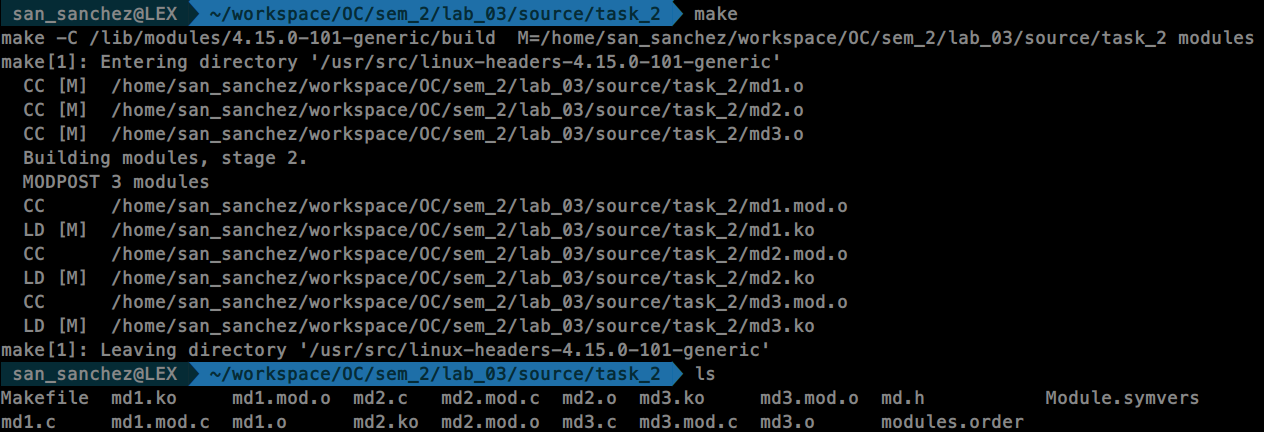
\includegraphics[scale=0.38]{data/image/task_2_1.png}
    \caption{Скришот результата работы make.}
\end{figure}

Попытка загрузки модулей в неправильном порядке:

\begin{figure}[H]
    \centering
    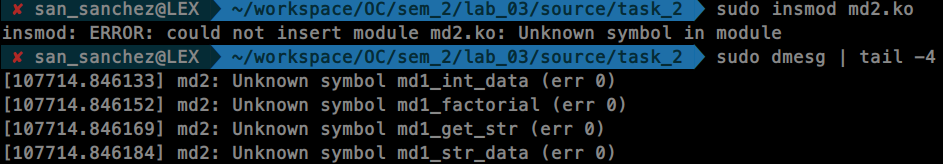
\includegraphics[scale=0.5]{data/image/task_2_2.png}
    \caption{Скришот результата работы insmod.}
\end{figure}

Ошибка возникла по причине того, что модуль содержит ссылки на неизвестные ядру имена.

Для правильной работы необходимо сначала загрузить md1.ko, а уже после этого - md2.ko.

Результат загрузки модулей в правильном порядке:

\begin{figure}[H]
    \centering
    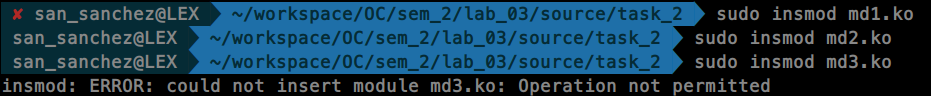
\includegraphics[scale=0.5]{data/image/task_2_3.png}
    \caption{Скришот результата работы insmod.}
\end{figure}

Демонстрация успешной загрузки:

\begin{figure}[H]
    \centering
    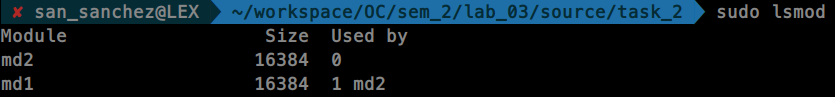
\includegraphics[scale=0.6]{data/image/task_2_4.png}
    \caption{Скришот результата работы lsmod.}
\end{figure}

Вывод dmesg:

\begin{figure}[H]
    \centering
    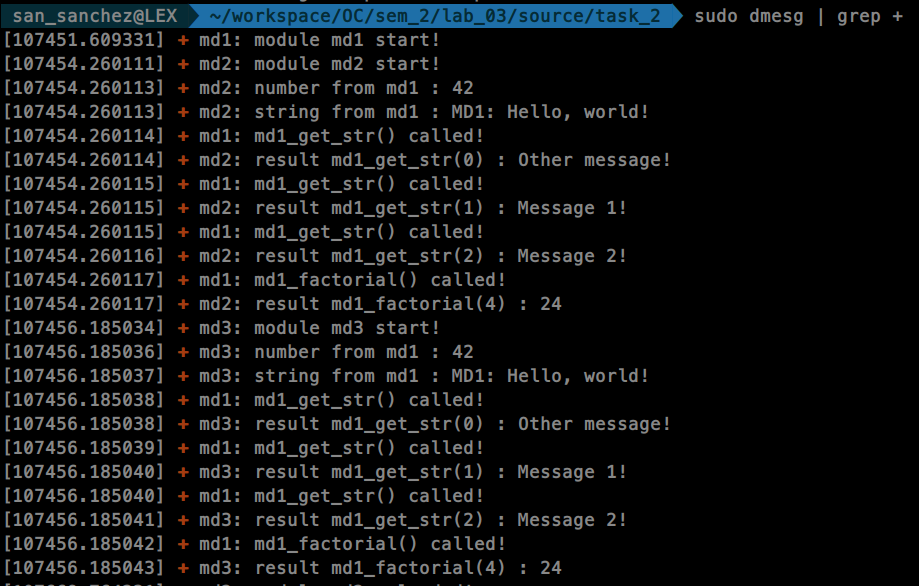
\includegraphics[scale=0.5]{data/image/task_2_5.png}
    \caption{Скришот результата работы dmesg.}
\end{figure}

Попытка выгрузки модулей в неправильном порядке также вызовет ошибку:

\begin{figure}[H]
    \centering
    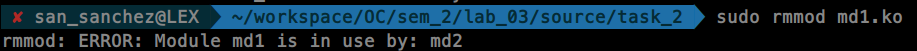
\includegraphics[scale=0.5]{data/image/task_2_6.png}
    \caption{Скришот результата работы rmmod.}
\end{figure}

Результат успешной выгрузки модулей:

\begin{figure}[H]
    \centering
    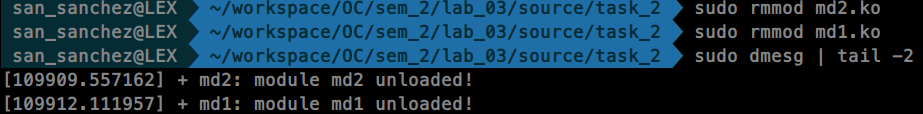
\includegraphics[scale=0.5]{data/image/task_2_7.png}
    \caption{Скришот результата работы rmmod.}
\end{figure}


